\section{CityScope Architecture \label{sec:cityscope_architecture}}

 {
  \subsection{Introduction}
  {
      The previous Chapter discussed the role of insights as a way to converge on urban places and issue in need for a change (see Chapter \eqref{ch:insight}). In CityScope, the exploration of \textit{change} is achieved by iterating through many design interventions and policies, using a range of Urban Human Computer Interaction (UHCI) methodologies, systems, and interfaces. The design of CityScope as an end-to-end ecosystem of UHCI components was developed over several years. At first, components were developed in silos, which forced CityScope projects to be tightly integrated and single-use (see, for example, CityScope BRT \eqref{sec:brt}). The system described in this chapter is of CityScope as a modular architecture, which by-design allows for the integration of different components, and their reuse in new projects. In order to communicate between the different parts of the CityScope system, a common data schema was developed (`CityScope Schema'). This schema is used to store, exchange, and define the data types and semantics of the different components. Figure \eqref{fig:cs_arch} illustrates the modular design of CityScope and the transfer of data using the Schema.
      \newline
      The rest of this section details the architecture of the CityScope ecosystem, discusses the design of the communication and storage service (`cityIO'); urban analysis microservices (`CityScope Modules'); as well as TUI (`CityScoPy') and frontend (`CityScopeJS') clients.
  }


  \begin{figure}[!htb]
      \begin{center}
          \includegraphics[width=1\textwidth]{chapters/transformation/cs_arch/figures/arch/cs_arch0.png}
      \end{center}
      \caption{
          CityScope Architecture. This diagram presents the data flow and different components of the CityScope architecture: (purple) Different modules control the inputs and CityScope Grid interaction; (blue) Upon interaction, cityIO VPC handles the transaction with different analytics modules; (green) When the computation phase is completed, the grid and analysis modules results are sent to output devices, either online (CityScopeJS, API), or onsite (projectors, monitors)
      }
      \label{fig:cs_arch}
  \end{figure}

  \subsection{Schema and Types System}\label{subsec:types_system}
  {

      \begin{figure}[!htb]
          \begin{center}
              \includegraphics[width=0.8\textwidth]{chapters/transformation/cs_arch/figures/arch/cs_arch1.jpg}
          \end{center}
          \caption{Type System and CityScope Schema. This diagram presents three examples of basic and more complex types as CityScope grid tiles, and how they are encoded in the Schema using LBCS and NAICS codes. (Figure: Luis Alonso, MIT)}
          \label{fig:type_sys_schema}
      \end{figure}

      The CityScope Schema defines a set of \textit{`types'} that are used to describe land-uses, urban functions, and purpose of fixed-size, rectangular geographical-units. These units can then be combined and arranged to represent complex urban environments over a CityScope intervention area, or the  \textit{`grid'}. Types are assigned to all cells in the grid, providing unified segmentation, scale, and a level of abstraction, that can be easily manipulated by users in both physical TUI and virtual interfaces. Cells within the grid can either be immutable or amendable, depending on the project specifications; At minimum, each tile must include one LBCS land-use, but most modules would require also one economic activity. The land-use data is based on the LBCS land-use classification system \cite{montenegro2012land}, and the economic activity data is based on the NAICS codes \cite{NorthAme86:online}\footnote{
          \textit{Land Use Classification Notation} or LBCS classification system includes activity, function, building type, site development character, and ownership constraints in each of its dimensions (for LBCS scheme breakdown, see \eqref{appendix:schema-description}).
          \newline
          \textit{Economic Activity Classification Notation} or NAICS are a standard used by Federal statistical agencies in classifying business establishments for the purpose of collecting, analyzing, and publishing statistical data related to the U.S. business economy. Codes are generated using a numerical classification outlined in the NAICS manual \cite{NorthAme86:online} (for NAICS scheme breakdown, see \eqref{appendix:schema-description}).
      }.
      Types may differ from one project to another, depending on the desired intervention or research question. For example, a CityScope project might include types associated with different levels of energy consumption, in order to asses how certain spatial arrangements can change energy usage.
      \newline
      In order to transfer Schema data between the different components of CityScope, a server system called `cityIO' was designed. The next section details the evolution and design of this system.
  }


  \subsection{cityIO}\label{subsec:csarch-cityio}
  {

      \begin{figure}[!htb]
          \begin{center}
              \includegraphics[width=0.5\textwidth]{chapters/transformation/cs_arch/figures/arch/cs_arch2.png}
          \end{center}
          \caption{cityIO V1: Data flow in the early version of cityIO.}
          \label{fig:cityio_v1}
      \end{figure}


      \textit{cityIO} is a CityScope service responsible for the communication between the different components of the CityScope ecosystem. cityIO maintains the current and - in some cases - the past state of CityScope instances, as well as preform other server-side tasks, such as security and user-logging. In 2015, cityIO first version was created with the sole purpose of supporting communication between a tangible user interface (TUI) and a handheld AR device. That version was developed using User Datagram Protocol (UDP), a fast yet unreliable packets-based communication \cite{richard1994tcp}. When users interacted with the CityScope TUI (for example, by moving a LEGO tile), a packet would be sent to the server, and then broadcasted to the AR devices (see Section \eqref{sec:cityscope_ar}). With each interaction, the virtual environment in these devices would react with updated visualizations and analysis. UDP presented several challenges: (i) Its data reliability was limited, and lost data packets caused inconsistent user experience, (ii) UDP was not scalable to web-apps due to security concerns. In 2016, an HTTP server-client system has been proposed to allow more scalable and reliable communication between elements of the CityScope ecosystem.

      \subsubsection{cityIO Ver. 1 (`15-`18)}
      {
          The first version of cityIO was using an HTTP protocol and a REST API, which exposed a simple data packet called \textit{CityScope Grid}. The grid was digital translation of a 2D array of objects, which represented the state of the CityScope TUI; With each user interaction, the grid would update, and sent to the server. The server then stored the grid, so that other microservices or devices could access it. By design, cityIO did not limit the access and modification of the grid by other microservices or devices, so that its state could be updated from all ends of ecosystem (i.e., analysis services, other TUI, etc.). The Grid was a JSON object which included a list of lists; Each element in the list had two numerical variables: $[type, rotation]$. The `type' is a numeric index of a list of land-uses\footnote{These land uses could be as simple as as `offices', `housing', or `road', or more complicated types, such as `offices for large companies with retail at the bottom two floors'}, and the `rotation' is the rotation of the physical tile (i.e., 0 - facing up, 1 - 90° rotation, etc.). As such, a client reading the grid, would assume that the tile $[t,r]$ at position $[i,j]$ is of type $type_t$ and rotated $rotation_r$. A typical data sample of the grid object is shown in the Appendix \eqref{appendix:cityio_output_format}. This cityIO version was built with in NodeJS, python, and later in GO.
          \newline
          \textbf{Usage:} The HTTP bidirectional communication enabled users to not only obtain the state of the CityScope TUI, but also interact and share their opinion during real-time CityScope design sessions. For example, users could select geo-located spots in the virtual grid (such as buildings, parks or roads) and add textual comment to the designs proposed by other users, done by simply extending the JSON object of that grid-cell (for example, see the AR application in Andorra at Section \eqref{sec:andorra-data-observatory}). This type of communication offered designers, decision-makers, and communities a way to participate in a shared physical-virtual design session.
          \newline
          \textbf{Limitations:} First, the lean data structure of the grid was not easily interpretable by other microservices or end-user devices. Each microservice would have to parse the grid object, based on predefined Knowledge of the way the grid was structured. This created inconsistency when some microservices were parsing the grid differently from others. Second, the TUI responsible to share the grids' state, was often triggered by external events, such as light bursts, or a slight movement of the TUI table. This created a torrent of data packets flooding the server, which was not scalable, and created a bottleneck in slow-moving microservices. These issues were addressed in the next version of cityIO.
      }



      \begin{figure}[!htb]
          \begin{center}
              \includegraphics[width=.65\textwidth]{chapters/transformation/cs_arch/figures/arch/cs_arch3.png}
          \end{center}
          \caption{Converting a site to the CityScope Schema: (a,b) designating and aligning an urban intervention site (c) `pixelation' of the site's land-use using the Schema (d) building the TUI for the CityScope context}
          \label{fig:voxel_to_schema}
      \end{figure}


      \subsubsection{cityIO Ver. 2 (`18-current)}
      {
          Amidst these challenges, the second version of cityIO was designed more as a real-time database than a massaging service. The main difference was the implementation of a new CityScope Schema, that was assuming no prior knowledge of the grid, the contextual area, or other baseline information. Instead, the schema was designed as a single JSON object, which hold key-value pairs for the entire data needed for a microserviced CityScope instance. The bare minimum key-value pair is of one \verb|GEOJSON| object called \verb|GEOGRID|, which included all necessary information to render the grid, including geo-location of each grid-cell, their types, and other properties (see examples ver.2 in Appendix \eqref{appendix:cityio_output_format}). Using this object, CityScope users, clients, and microservices could understand the structure of the grid, and parse it in a user-friendly way.
          \newline
          Unlike the first version of cityIO schema, \verb|GEOGRID| is an immutable object, which should not be changed by other microservices. Instead, a mutable object called \verb|GEOGRIDDATA| was introduced, in which only the core properties of each grid-cell are stored. This object is smaller than \verb|GEOGRID|, and is constantly updated by the TUI or other microservices, as needed. The logic behind this design is to maintain a single source of truth for the grid with \verb|GEOGRID|, thus always preserving the initial `tabula-rasa' state of the site in question.
          \newline
          Additional key-value pairs in the root of the CityScope Schema are defined as `CityScope Modules' (see Section \eqref{subsec:cs-modules}), which are the aggregated analysis results of different computational modules or microservices. The next section describes how CityScope modules analyze and evaluate the grid data, and share their results with cityIO.
      }
  }

  \subsection{Microservices and Modules}\label{subsec:cs-modules}
  {
      As discussed in Section \eqref{sec:cityscope_architecture}, CityScope architecture is based on \textit{microservices}, which are a set of computer services that are designed to run independently of each other. The microservices are designed on different platforms and operating systems, so that each service can operate on its designated environment \cite{balalaie2016microservices}. This architecture stems from the idea that each microservice can be designed independently, as long as a shared terminology exist.

      \subsection{Microservices}
      {
          In the context of city-planning and spatial analysis, the CityScope ecosystem requires a wide spectrum of microservices; From straightforward calculations of square footage, to complex noise, energy, or traffic simulations. If in early stages, CityScope was composed of a single service for a single instance (such as the zoning simulation in CityScope Playground, see Section \eqref{sec:cityscope_playground}), the microservices design would allow for each CityScope to preform multiple tasks and analyze various aspects in concurrency.
          \newline
          Another motivation for the development of a microservices architecture, is the need to support the extension of CityScope interfaces beyond the TUI. Decoupling UI, feedback, and analysis microservices allows to add new interfaces, modules, and visualization aids without having to update the existing hardware or software. For example, projects like CityScope Corktown can be fully accessed on a web-browser, where CityScope Ho Chi Minh City would utilize a physical interface, all the while running the same underlying microservice architecture.
          \newline
          Lastly, the microservices architecture is designed to be easily extensible. Since a major aspect of CityScope is open-source and collaborative development, contributions to either frontend, backend, or individual microservices is made possible using detached components. In that manner, the teams working on CityScope Grasbrook (see Section \eqref{sec:grasbrook}) were able to extend the CityScope ecosystem to include new microservices, add functionality to existing ones, as well as redesign the frontend and TUI components as needed.
      }


      \begin{figure}[!htb]
          \begin{center}
              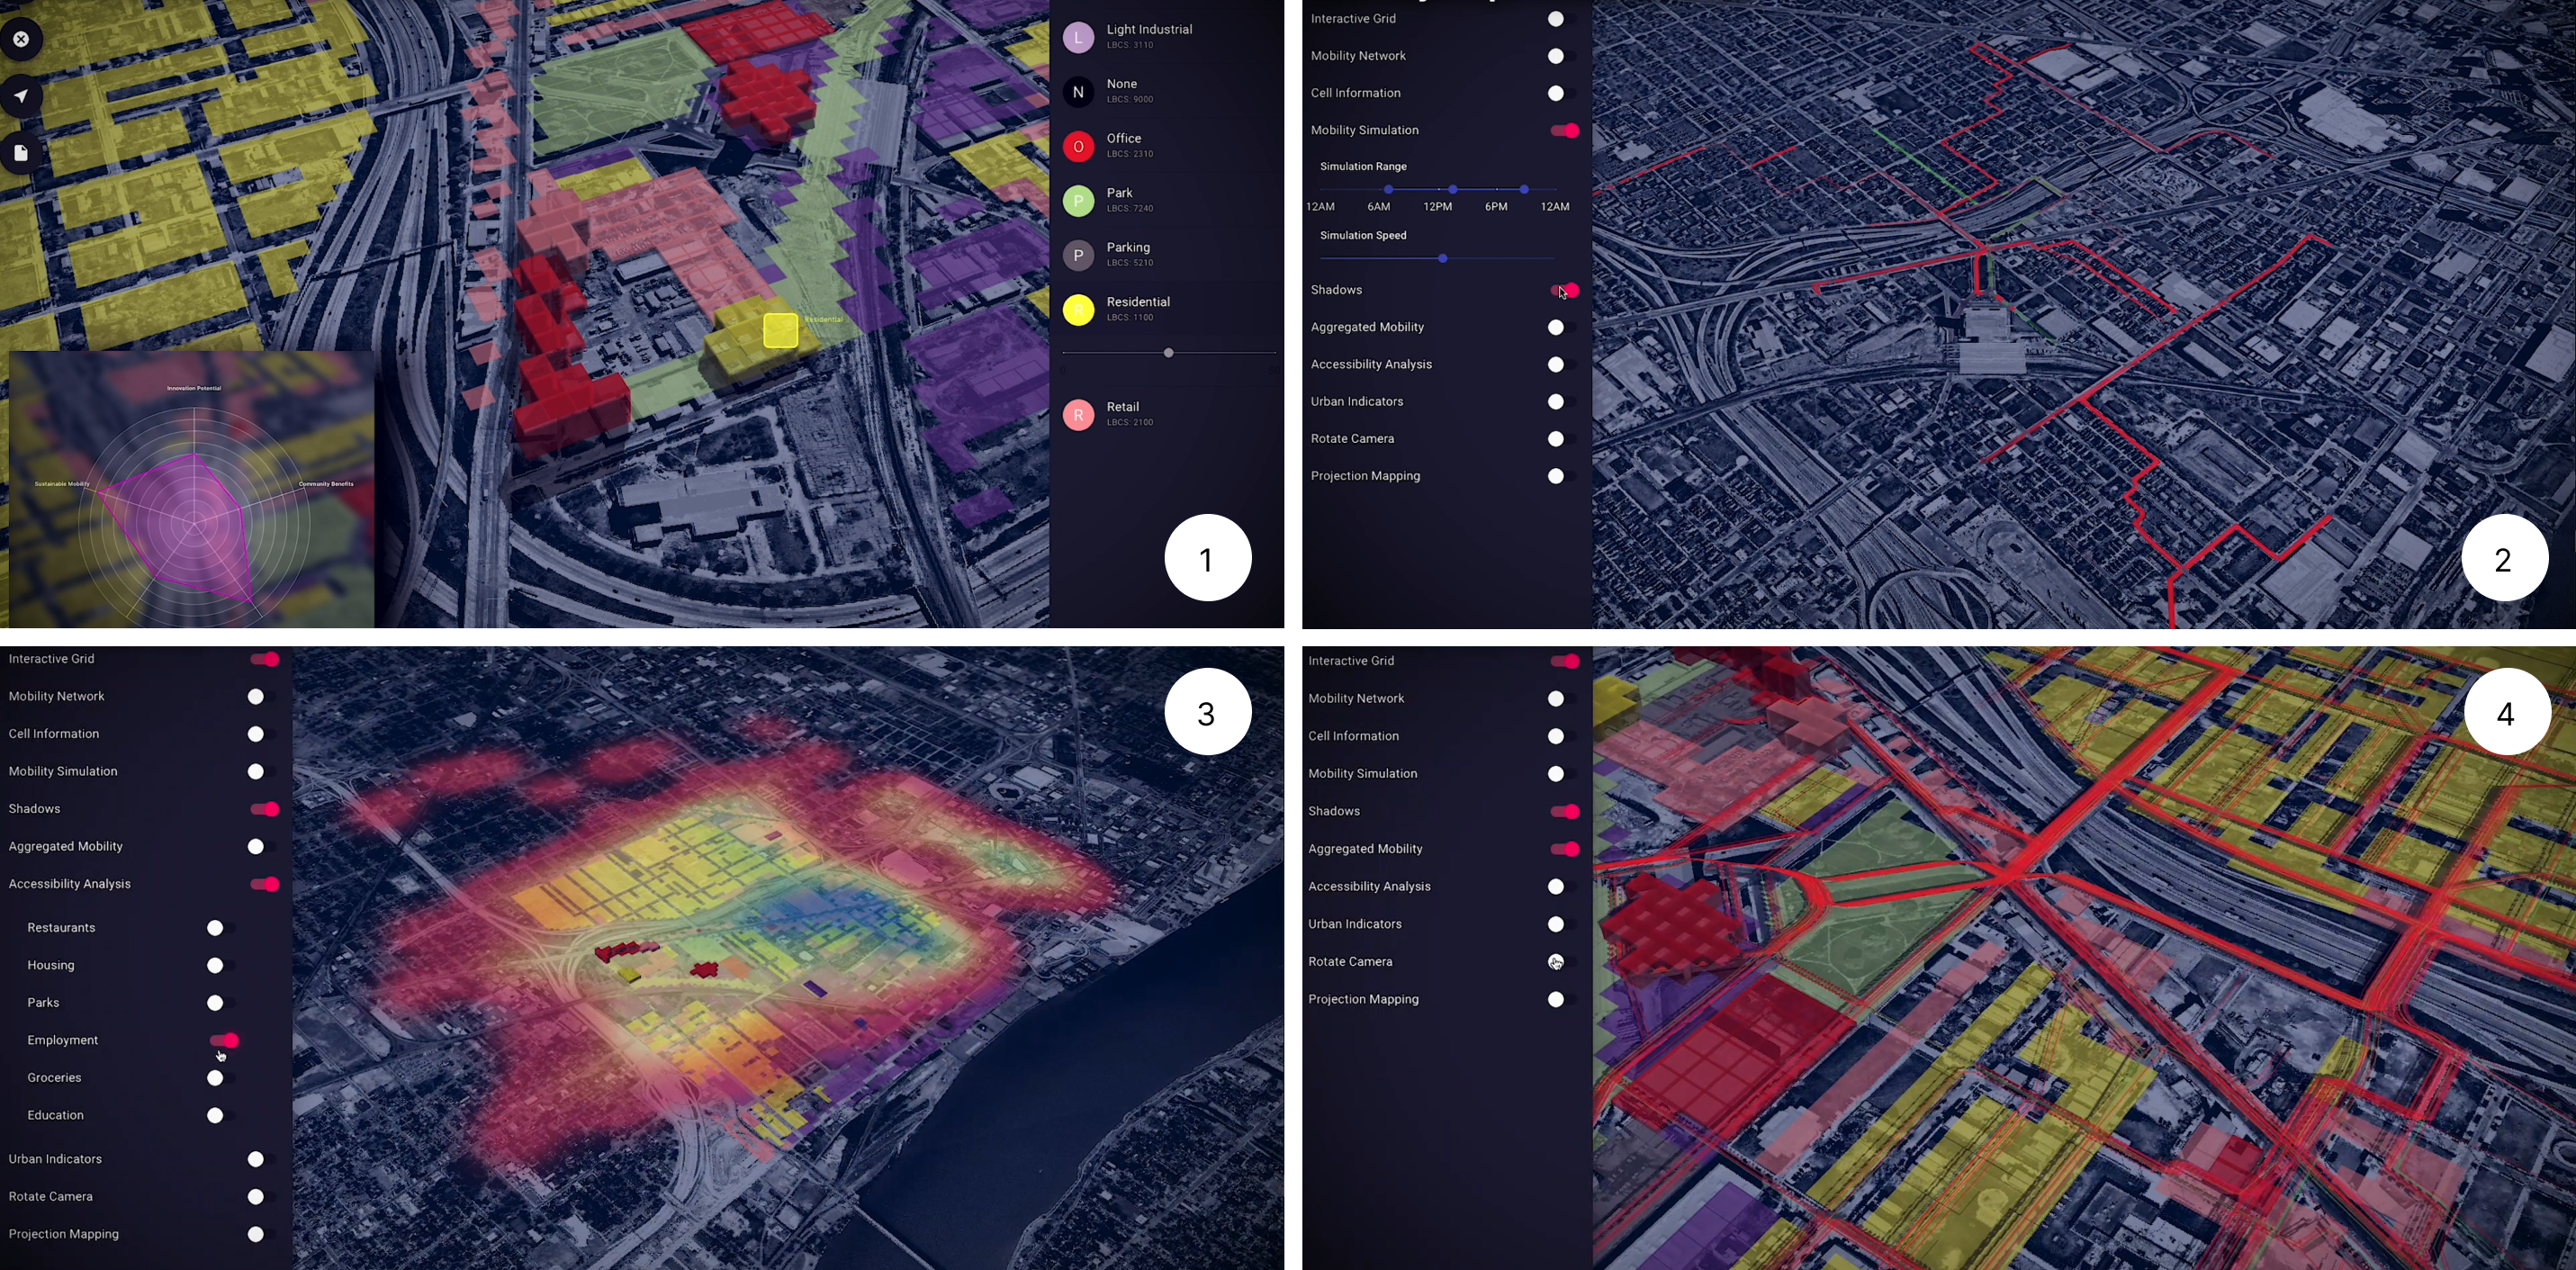
\includegraphics[width=1\textwidth]{chapters/transformation/cs_arch/figures/csjs/csjs_0.png}
          \end{center}
          \caption{CityScopeJS interface. Similar to the TUI versions of CityScope, users interaction is design to be simple and intuitive. Interactions are sent to the cityIO analysis modules, and their responses are then displayed spatially as heat-maps, trips, or graphically as charts and data visualizations. (1) CSjs grid design using a `paintbrush' gesture; (2) animated results of mobility analysis module; (3) results of accessability heatmap to employment and other urban attributes; (4) accumulated traffic results and mobility mode for each road segment.}
          \label{fig:csjs}
      \end{figure}



      \subsection{Modules}
      {
          CityScope Modules is a collection of backend microservices which preform the analysis for a CityScope project. Every time a user interacts with the CityScope interface (via virtual or physical UI), their \verb|GEOGRIDDATA| state is updated on the cityIO server; Modules are constantly listening to these changes, and are triggered to preform analysis with each change.
          When a CityScope module completes an analysis, its results are sent back to cityIO, so that the frontend, and other modules, would have access to it. The analysis results are called `indicators', which can be any of numeric, heatmap, simulation, or textual representation. Numeric indicators are usually displayed as a chart (bar, radar, etc. See Section \eqref{sec:cityscope_volpe}). Heatmap indicators are geo-located (points, lines, or polygons) which are displayed as layers directly on the CityScope table. Simulations are also displayed on the table but are the result of a temporal analysis (such as ABM, mobility simulation, etc) and are therefore displayed as a dynamic layer.
          \newline
          Some modules' results are not directly visualized on the CityScope interface. Instead, these modules would only compute so that other modules could use their results, as part of their analysis. For example, a CityScope table dedicated to the analysis of noise in a new development site, would use mobility simulation to indicate the types and volume of vehicles traversing through the area. The results of this mobility module would not be used for visualization, but instead would become available for the noise module itself. This structure allows greater complexity and dependency of analysis modules. To ensure all modules are synced with the current state of the \verb|GEOGRIDDATA|, cityIO produces a unique hash for each grid state (see Appendix \eqref{appendix:cityio_output_format}). The next section describes how modules' results and user interaction are combined in the CityScopeJS frontend.
      }
  }



  \begin{figure}[!htb]
      \begin{center}
          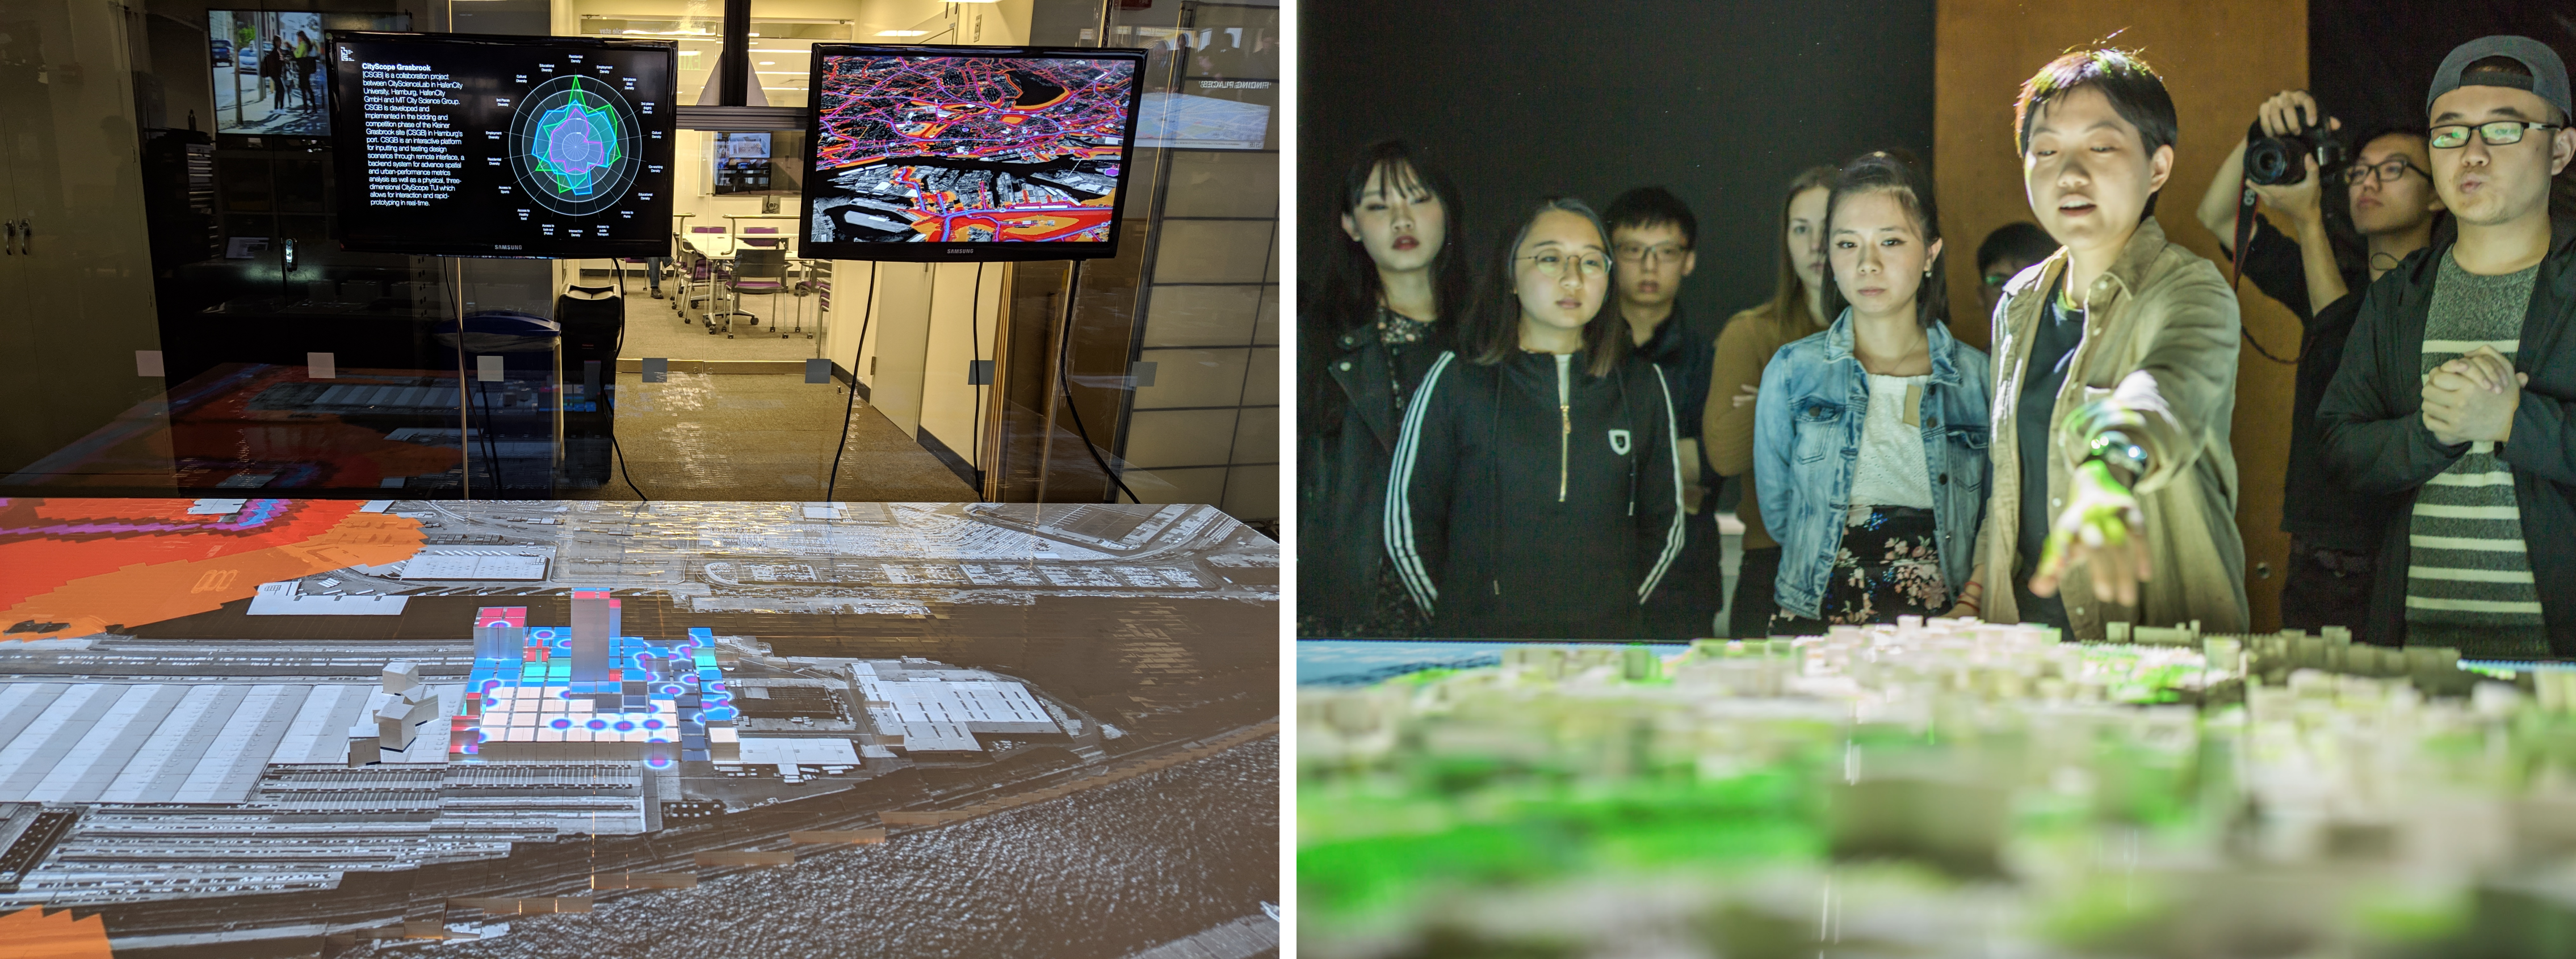
\includegraphics[width=1\textwidth]{chapters/transformation/cs_arch/figures/csjs/csjs_1.png}
      \end{center}
      \caption{CityScopeJS usage in tangible interfaces. (left) CSjs for the Grasbrook project in Hamburg \eqref{sec:grasbrook}; (right) an early version of CSjs for a student workshop in Aalto University, Espoo, Finland.}
      \label{fig:csjs_tui}
  \end{figure}

  \subsection{CityScopeJS (`CSjs')}
  {
      CityScopeJS\footnote{stands for CityScope Javascript or `CSjs' in short.} is the unified online frontend for the CityScope ecosystem. CSjs is designed to combine the most common use-cases for any CityScope instance: initiation, interaction, visualization, and feedback. CSjs allow users to examine different urban-design alternatives and understand their impact, through a range of KPIs, metrics, visualizations, and charts. It can be used as a standalone online tool, or in combination with TUI in an physical setting. Using its interface, users can edit a grid and change land-uses, buildings, open spaces or transport routes, as well as amend their properties and attributes. As soon as the user concludes their design session, their grid state is sent to cityIO for calculations by the modules. When these are computed, CSjs pulls the new analysis results from cityIO, and displays them on the interface. CSjs is built with ReactJS and DeckGL \cite{ReactAJ49:online,deckgl17:online}. The rest of this section describes the features of CSjs.

      \begin{figure}[!htb]
          \begin{center}
              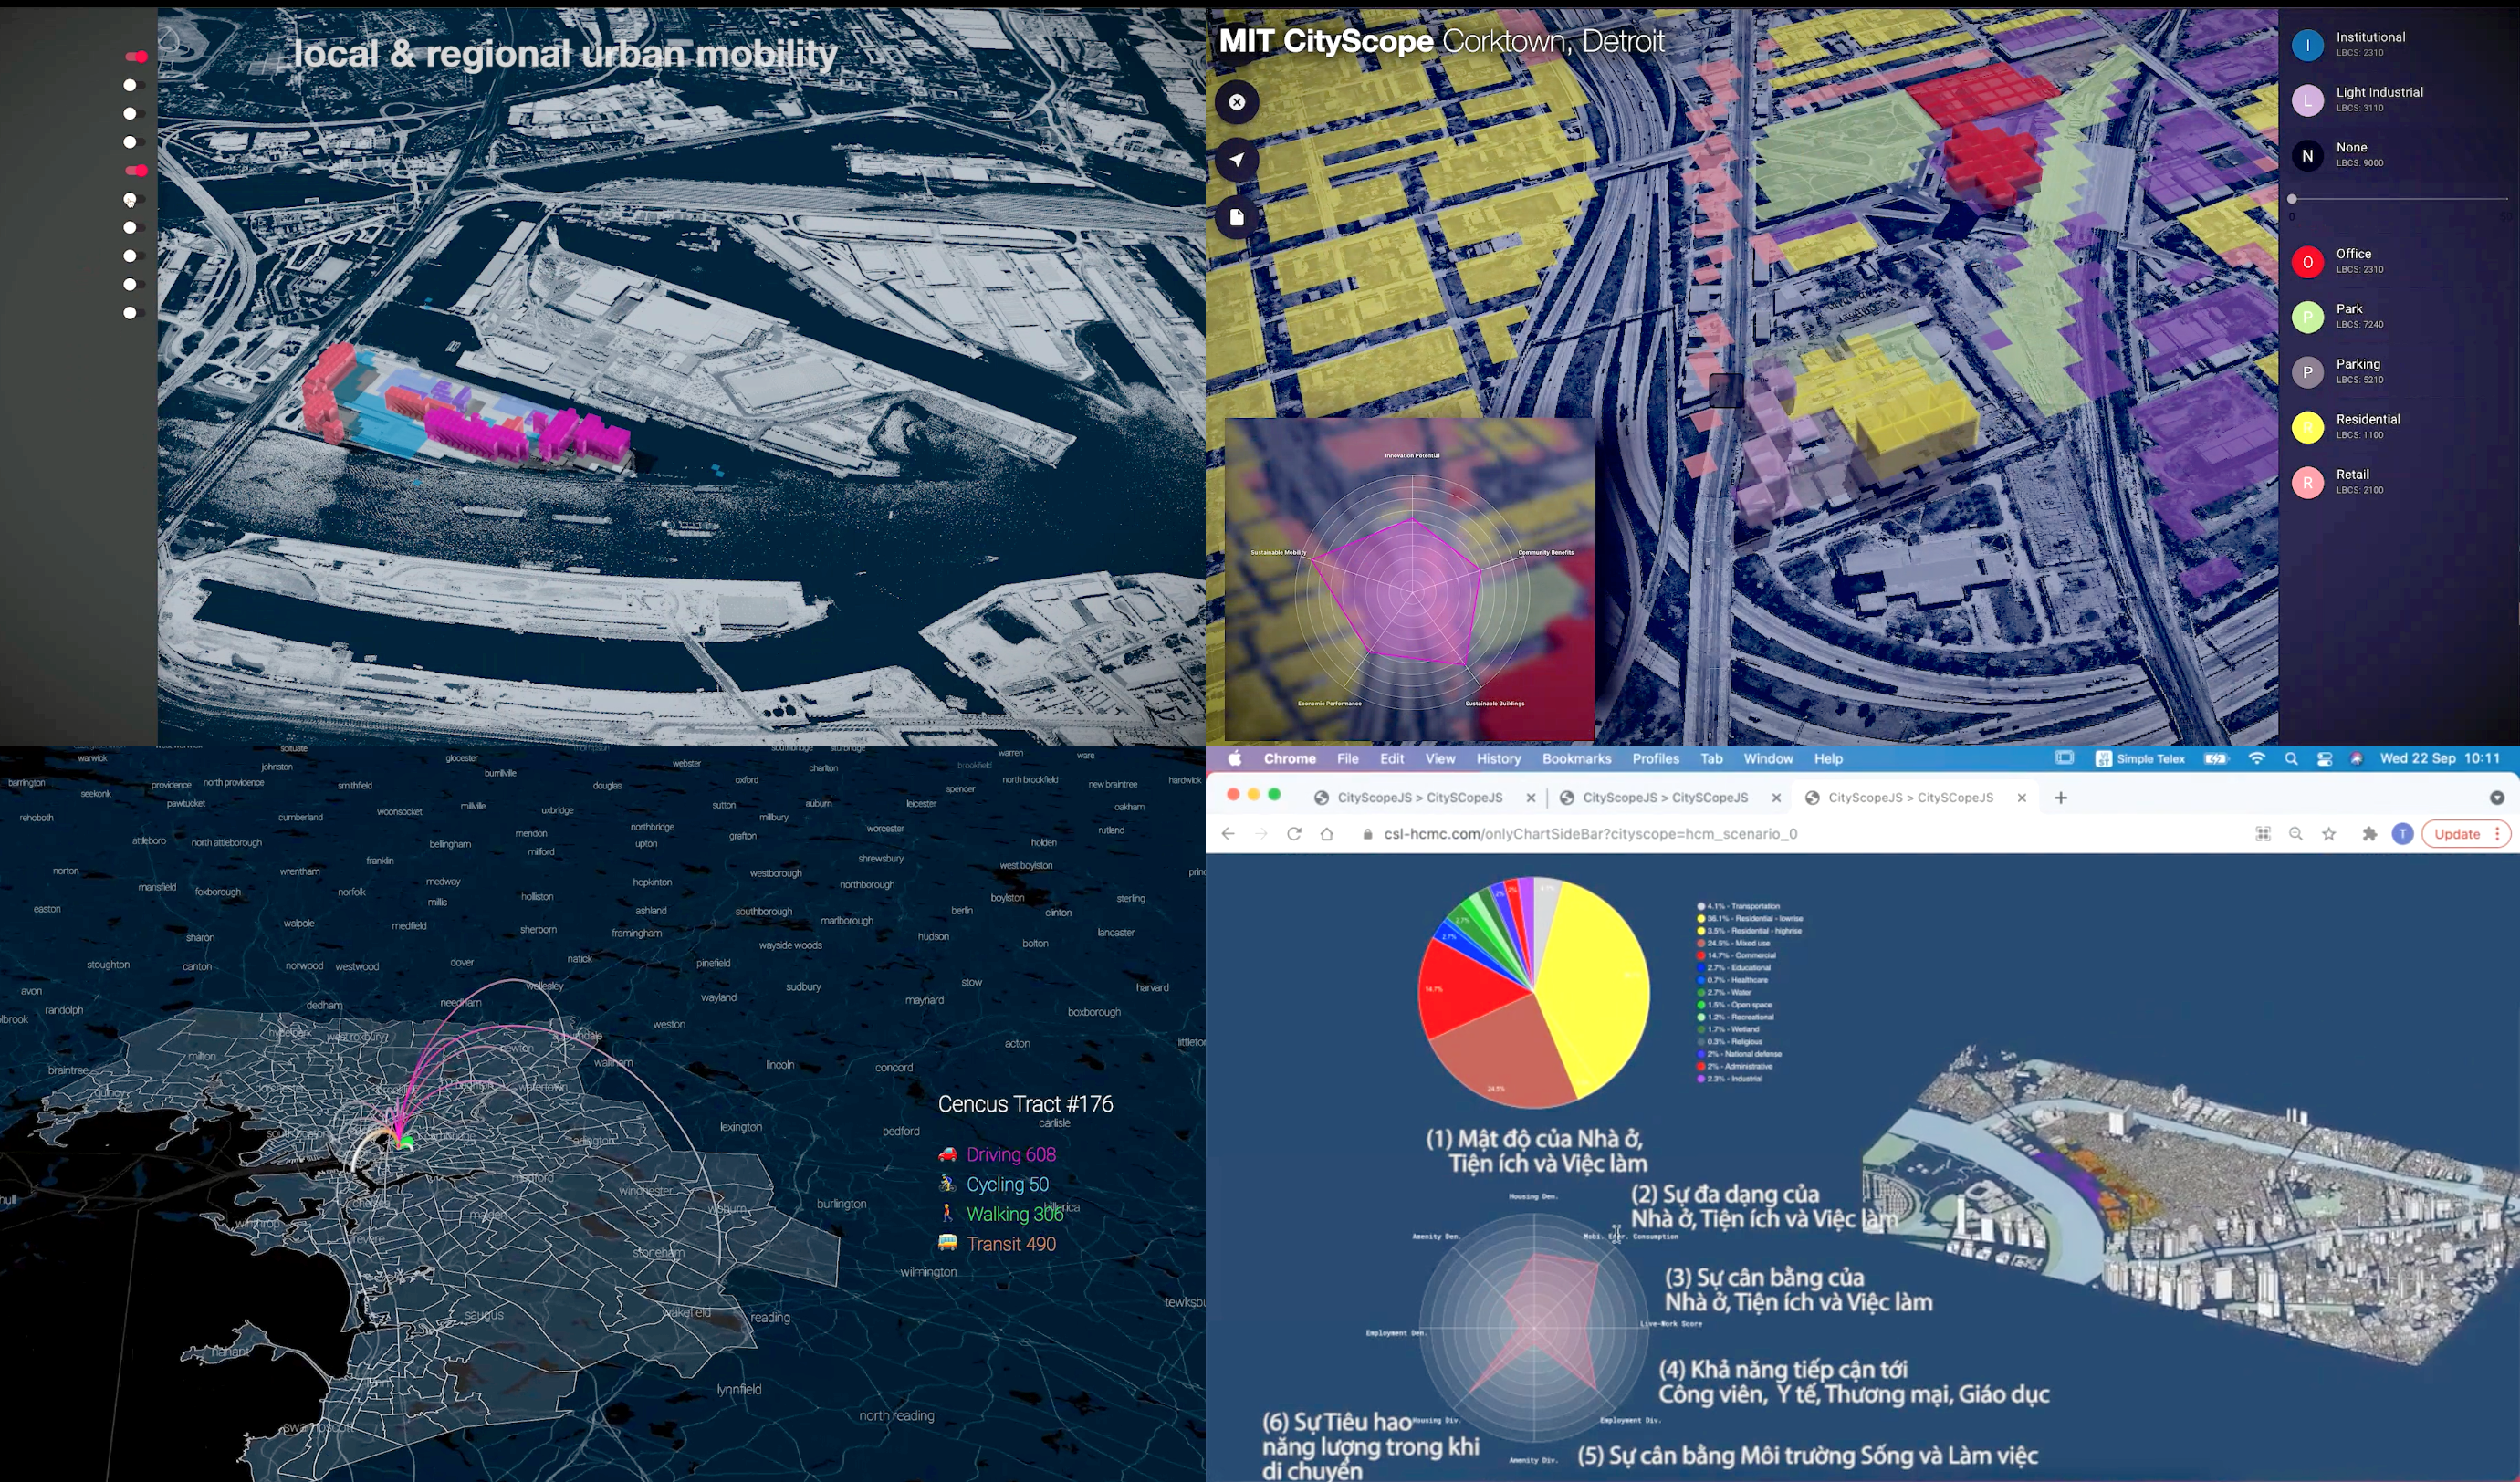
\includegraphics[width=1\textwidth]{chapters/transformation/cs_arch/figures/csjs/csjs_2.png}
          \end{center}
          \caption{CityScopeJS case-studies. (top-left) CSjs for the CityScope Grasbrook project in Hamburg, 2019 \eqref{sec:grasbrook}; (top-right) CSjs for the Corktown project in Detroit, MI, 2020; (bottom-left) CSjs for the CityScope MoCho, 2018 \eqref{sec:cityscope-mocho}; (bottom-right) CSjs for the Ho Chi Minh City project in Vietnam, 2021.}
          \label{fig:csjs_versions}
      \end{figure}


      \subsubsection{CSjs Features}
      {
          CSjs exposes three main features: \textit{Grid Editor}, \textit{Playground}, and \textit{Projection}. The CSjs Grid Editor is a helper tool to initialize and bootstrap new CityScope projects. It allows the creation of (i) a CityScope endpoint on cityIO (with a dedicated URI); (ii) a virtual, geo-located, 3D, and editable CityScope grid; and (iii) a list of `types' to be used in the design of this CityScope instance. The definition of types and their attributes strictly follows the aforementioned CityScope Schema (see Subsection \eqref{subsec:types_system}).
          \newline
          The \textit{CSjs Playground} is where users interact with the predefined CityScope grid. The interface is built to allow for simple, intuitive, and real-time intervention with the grid setup and land-uses, mimicking the ease of use of a traditional LEGO TUI. Unlike other CAD and planning tools, CSjs interface features minimal functions, toolbars, or menus, and is designed to be used with simple hand gestures on various devices, from an 9 ft TUI table, to a handheld cellphone.
          \newline
          Lastly, the \textit{CSjs Projection} is a tool to visualize the results of the CityScope modules on a TUI interface, such as a tangible grid. This is a passive presentation tool, that listens and renders updates directly from cityIO, without user interaction. This tool uses non-affine projection mapping (homography algorithm) that is designed to render the CityScope Grid and modules results on a physical interface using projectors.
      }

      \subsubsection{CSjs Case Studies}
      {
          CSjs development became a standalone effort in 2019, but was preceded by several projects and experiments since 2017\footnote{Such as CityScope MoCho, see Section \eqref{sec:mocho_api}}. The goal of these was to test the feasibility of web-based CityScope instances. With the increased power of web-based rendering, GPU acceleration, and faster computation, it became clear that many aspects of the CityScope ecosystem could be migrated to the web.
          \newline
          The development of CSjs was boosted by the CityScope Grasbrook project, which presented a real-world use-case for an online, distributed, and collaborative urban-design tool (see Section \eqref{sec:grasbrook}). since 2017, the majority of CityScope projects were built on top of CSjs, such as the Grasbrook, Corktown, EPA, Ho Chi Minh City, Guadalajara, and others. In some cases, developers built their own custom modules, frontend components, or connected CSjs to other TUI. For example, the RoboScope\footnote{see \url{https://www.media.mit.edu/projects/roboscope/overview/}}, an actuated TUI inspired by the MIT Tangible Media inFORM table \cite{follmer2013inform}, uses CSjs to link its TUI to the rest of the CityScope ecosystem. The next subsection describes how other TUI and interfaces are integrated in CityScope.
      }
  }

  \begin{figure}[!htb]
      \begin{center}
          \includegraphics[width=1\textwidth]{chapters/transformation/cs_arch/figures/cspy/cspy_0.jpeg}
      \end{center}
      \caption{CityScope TUI. Physical 3D urban models, scanning module, feedback monitors and projection scheme. Variations of this setup were used in many CityScope projects.}
      \label{fig:cspy_tui}
  \end{figure}

  \subsection{CityScoPy}\label{subsec:csarch-cityscopy}
  {
      CityScoPy is a TUI library for CityScope written in Python. It is designed to recognize interactions with physical objects equally distributed over a 2D grid (such as LEGO tiles), and send the scanning results as a JSON object to cityIO (see Appendix \eqref{appendix:cityio_output_format}, \eqref{appendix:cityscopymethods}). CityScoPy exposes several functionalities, such as keystoning, scanning, and sending data to different endpoints, as part of the microservices architecture of CityScope. CityScoPy is built in Python and OpenCV for image processing \cite{opencv_library}.


      \begin{figure}[!htb]
          \begin{center}
              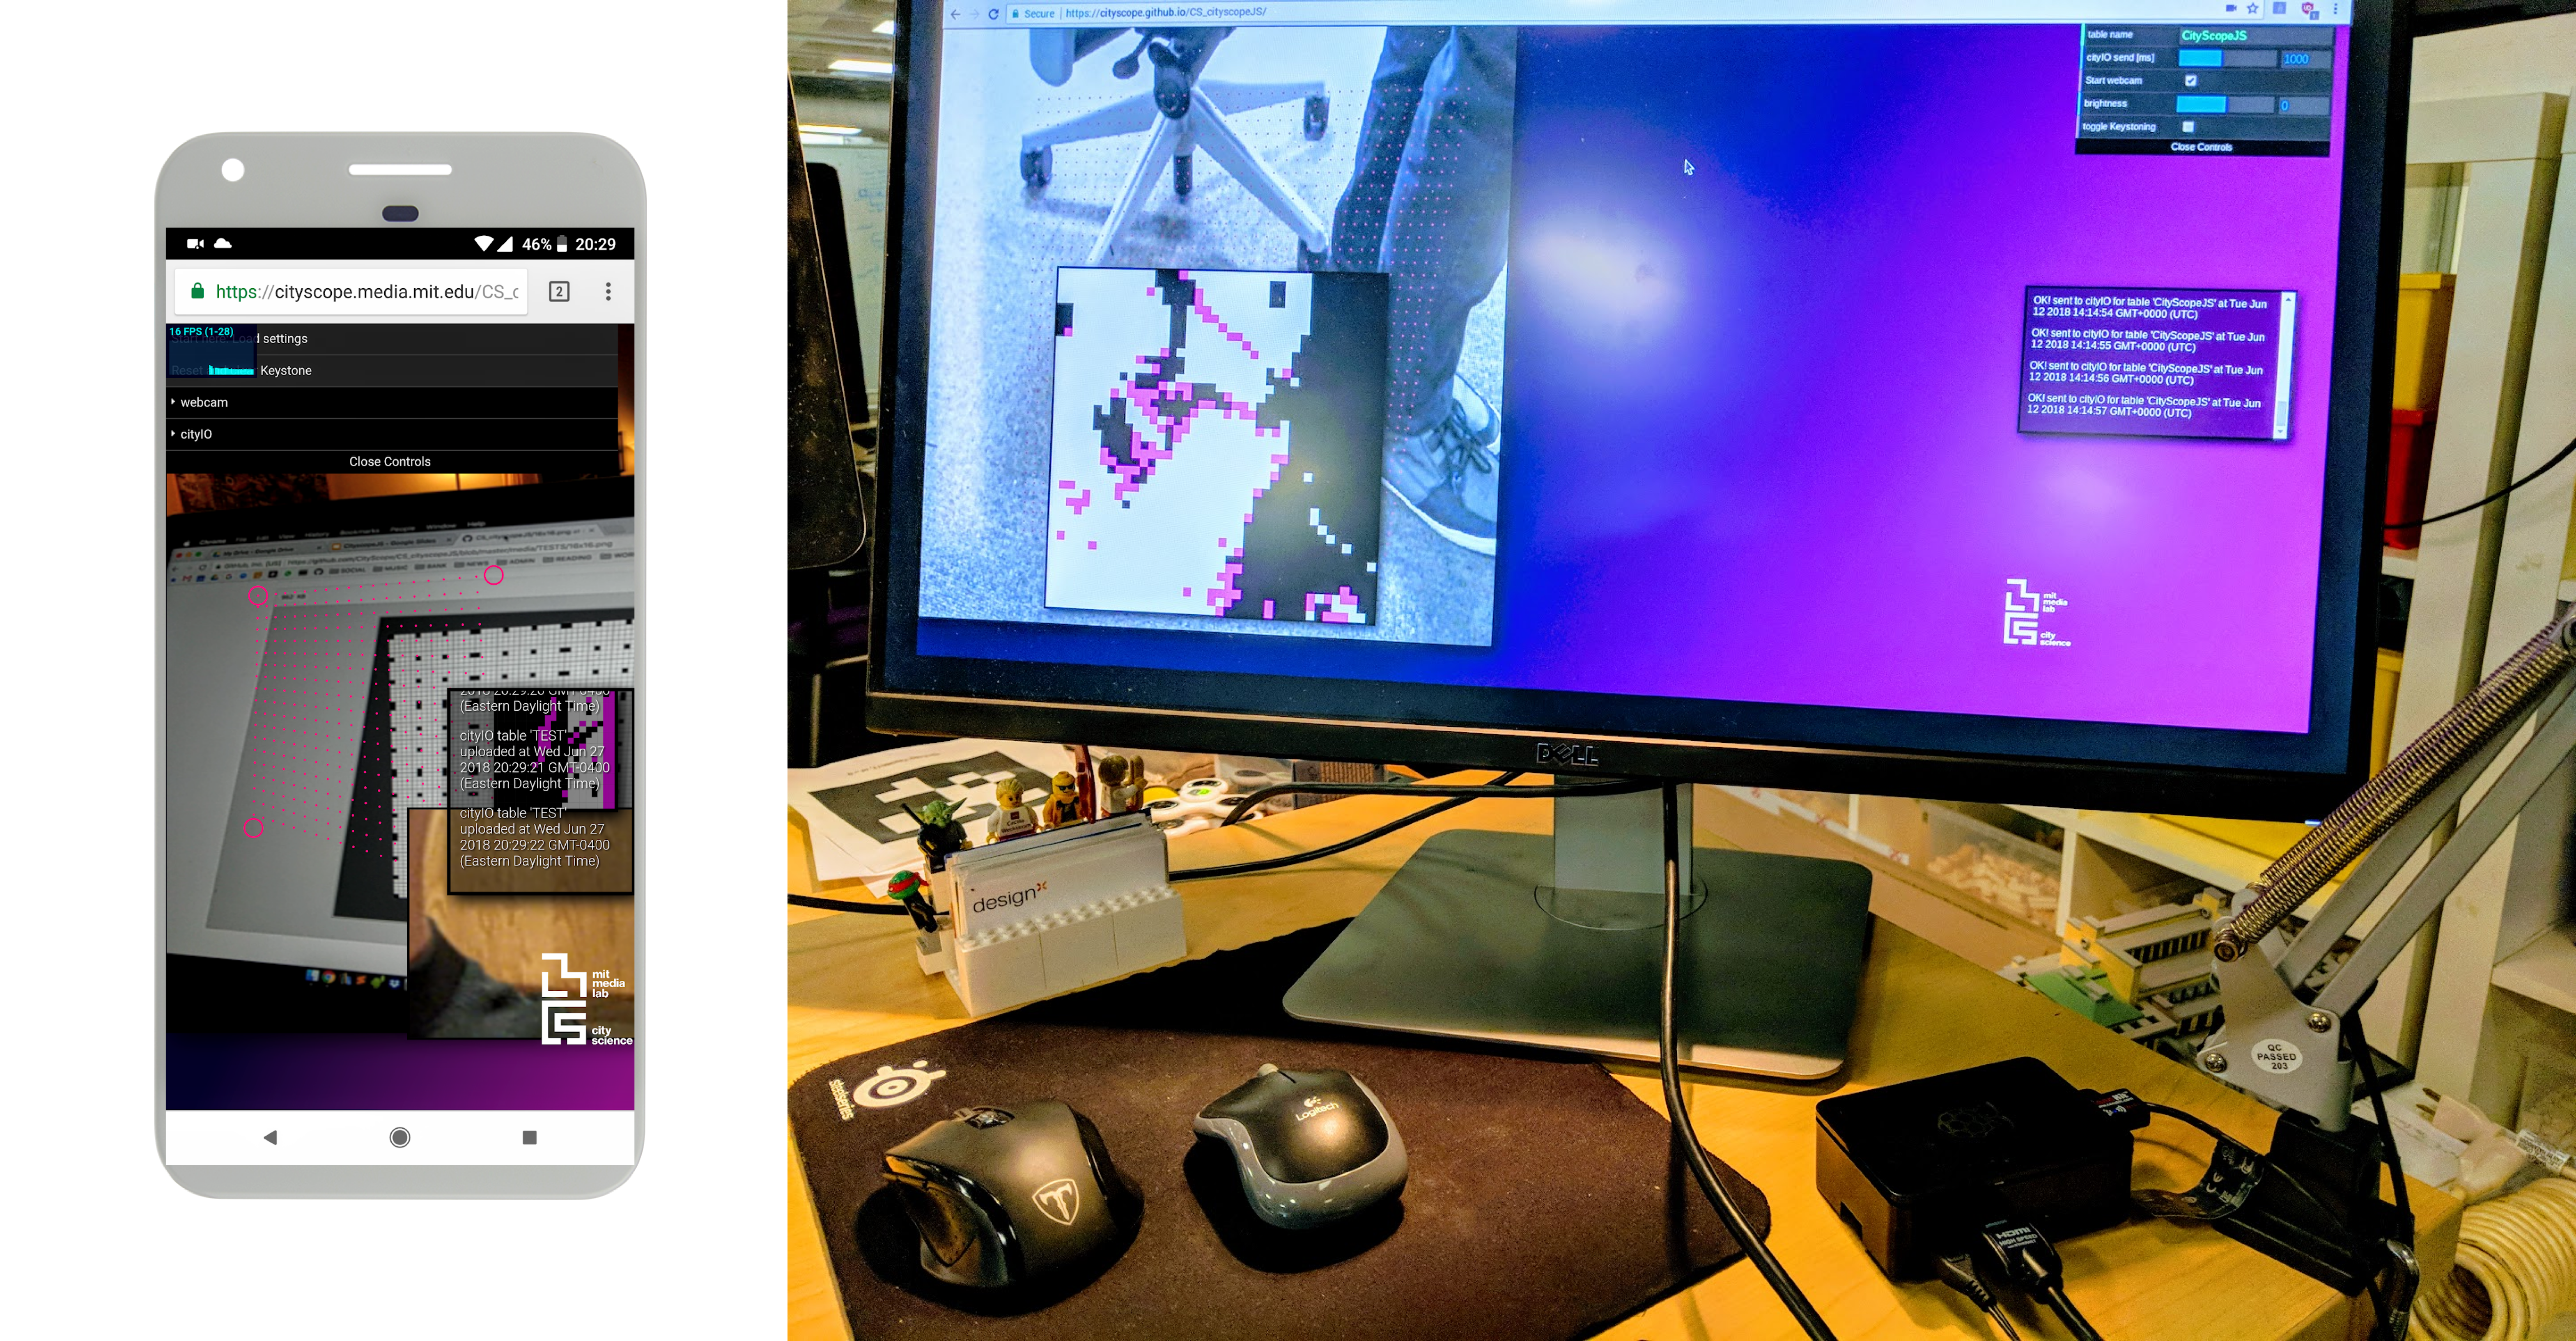
\includegraphics[width=1\textwidth]{chapters/transformation/cs_arch/figures/cspy/cspy_2.png}
          \end{center}
          \caption{CityScoPy scanner in action. This version of CityScoPy was created in vanilla Javascript to run on low-tier devices, such as cellphones or Raspberry-Pi with a basic web browser. Later versions were written in Python for faster scanning of larger grids.}
          \label{fig:cspy_scan_in_action}
      \end{figure}

      \subsubsection{Background}
      {
          CityScoPy is part of a long line of scanning tools developed over the years to support TUI for spatial analysis. Sensing the location of physical objects on a tabletop was prototyped in the exhibition ``Unbuilt Ruins''\footnote{By Kent Larson, displayed in Penn Architecture Archives (1999) and at `The Un-Private House' in the MOMA, NYC (1999)}, which featured digital-physical objects poised on top of a Louis Kahn's building blueprint \cite{sparacino1999technologies}. As users repositioned the objects, an array of projectors reviled rendered images associated with that object's location. Similar ideas were developed in the SandScape table \cite{ishii2004bringing}, where a digital relief of physical objects was captured in real-time using a top-down scanner. Since 2013, several scanning methods were developed by the CityScope team to capture physical objects and use them to simulate intervention and perform urban analysis \cite{Hadhrawi2016, zhang2017citymatrix, aldawood2014interaction}. These tools all shared the idea of scanning an array of predefined set of objects from beneath a translucent tabletop. The objects types were differentiated using colorful LEGO pieces, and the scanner was designed to recognize the objects' type and locations as users interact with them.
      }
      \subsubsection{Motivation and Design}
      {
          \begin{figure}[!htb]
              \begin{center}
                  \includegraphics[width=1\textwidth]{chapters/transformation/cs_arch/figures/cspy/cspy_3.png}
              \end{center}
              \caption{Example of a CityScoPy scanning result. The grid is scanned for binary values, and a 2D matrix is created to represent the grid cell. For each cell, a key-value pair search is conducted to find the corresponding type in the CityScope Schema.}
              \label{fig:cspy_results}
          \end{figure}

          CityScoPy was developed in order to improve several shortcomings in previous CityScope scanners: (i) \textit{Speed:} CityScoPy was designed to handle larger and more complex CityScope grids than before (see \eqref{subsec:vople_cityscope})\footnote{When tested on a 2015 Macbook Pro, CityScoPy scanned a grid of 100x100 4x4 LEGO tiles (total of 160000 scanned items) at 40fps.}. (ii) \textit{Versatility:} CityScoPy introduced a simple binary code, in which each of the LEGO studs of a 4x4 tile would be considered as either white or black\footnote{For example, a pattern with 4 white dots in the top-left corner and black in the rest would be [1,1,0,0,1,1,0,0,0,0,0,0,0,0,0,0].}. Using hues at the edges of the color gamut simplified the scanning algorithm, while still yielding $2^{16} = 65536$ unique permutations. This offered greater flexibility than the previous versions, while maintaining a simple way to differentiate types. (iii) \textit{Stability:} Previous CityScope scanners used a combination of colorful objects to identify types. These were proven unstable, since the scanner would tend to observe the same color at different parts of the tabletop as different RGB values. Since CityScoPy uses a binary code to define each type, the possibility of errors are reduced to the edge cases in the center of a gray-scale gamut. Additionally, the scanning algorithm captures and averages an array of 10x10 pixels for each scanning point, in order to reduce the potential of a faulty reading due to hazing or light bursts.
      }
      \subsubsection{Use-cases}
      {
          CityScoPy was adapted for several projects in HafenCity University, including the SmartSquare \cite{bley2020smartsquare} and CityScope Grasbrook \cite{baeza2021cityscope}. It was also used in several City Science network labs, such as Shanghai, Aalto, Guadalajara, and Jerusalem. At MIT, it was used for CityScope MoCho \cite{doorley2019s}, DeepScope \cite{noyman2020deepscope}, among others. In 2018, CityScoPy was used as part of an interactive installation for `The Road Ahead: Reimagining Mobility' exhibition in the Cooper-Hewitt Museum of Art, NYC \cite{CityScop40:online}. This CityScope artistically featured two extreme versions of a future with driverless cars: In one scenario, streets are dominated by vehicles which lead to congestion and anxiety; The other is a more vibrant city, where the benefits of walkability, mixed-use, density, and equity increase. In this context, CityScoPy allowed visitors to playfully interact with a fictional NYC-like urban grid, and impact the density and organization of the urban-scape in these two scenarios.
      }
  }

  \subsection{CityScopeAR}\label{sec:cityscope_ar}
  {
      \subsubsection{Introduction}
      {
          As discussed in Section \eqref{sec:cityscope_architecture}, the CityScope system design allows new ways to interact, visualize, and extend CityScope beyond the limitation of physical objects. CityScopeAR is a mixed-reality interface for CityScope, designed for remote yet collaborative urban-design processes. CityScopeAR builds on prior art using mixed-reality devices for CAD and urban-planning purposes (see Chapter \eqref{chapter:introduction}). The goal of CityScopeAR is to use hand-held devices such as smartphones, tablets, AR glasses, or VR headsets, and create a virtual environment that extends the tangible interface of CityScope, allowing users to interact with both the physical world and its virtual representation.
      }

      \subsubsection{System Design}

      {
          As discussed above in Section \eqref{subsec:csarch-cityscopy}, CityScope TUI tend to include a 3D urban model, projectors, and sensors to detect user interactions. Previous usability studies found several shortcomings in these setups \cite{Noyman2015power, Alrashed2015}: First, CityScope tables use flat-top tangible pieces projected with symbols and colors. In active participatory sessions, tables tend to get obstructed throughout most of the session, thus not communicating information as needed. Second, is the challenge of mixing different layers of information onto a single TUI; In user studies (see Section \eqref{sec:brt}), users requested different data layers to be displayed simultaneously. For example, experts might want to view traffic simulation, while member of the community wish to view the noise analysis layer. Lastly, CityScope TUI had no mechanism to systematically collect, store or display users' input and feedback. As shown in the Boston BRT project \eqref{sec:brt}, traditional surveys were used to collect users' feedback. All these suggested that alongside the CityScope TUI, additional representation and interaction methods should be explored.
      }

      \begin{figure}[!htb]
          \begin{center}
              \includegraphics[width=1\textwidth]{chapters/transformation/cs_arch/figures/ar/ar_2.png}
          \end{center}
          \caption{CityScopeAR extends the TUI with additional layers of analytics, data, and public participation. (left) CityScopeAR in Andorra used to collect user input concerning planning and urban development \eqref{sec:andorra-data-observatory}. (right) CityScopeAR for Boston BRT `Street Scale', showing traffic stats and impact on street area in accordance to the different BRT system type \eqref{sec:brt}.}
          \label{fig:csar_two_examples}
      \end{figure}


      \subsubsection{CityScopeAR Prototypes}
      {
          The first iteration of CityScopeAR was prototyped in 2015; A Macbook laptop displayed spatial layers that were mapped to the extents of a CityScope TUI using a set of colorful markers at the edges of the table. These data layers included physical elements (such as 3D building facades, sunlight, shadows, and vegetation), as well urban data layers (such as spatial analysis, heat maps, or interactive points of interest). This tool was developed using Unity and Vuforia SDK \cite{UnityRea35:online}, which were later replaced by Google's ARtoolkit and Nexus 9 tablets. In 2016, development of CityScopeAR shifted to the Google Tango Project; Tango devices allowed better object recognition and preflight area-learning, which was effective in challenging light condition imposed by CityScope projections. However, Tango's low market penetration put this development effort to an end in early 2017 \cite{kastrenakes2017google}. Later, CityScopeAR was developed with Google ARcore and Apple ARkit \cite{oufqir2020arkit}, which are now available on most mobile devices.
      }

      \subsubsection{Tests and Deployments}
      {
          \textbf{BRTCityScopeAR for Boston BRT:} CityScopeAR was developed alongside several key CityScope projects, which offered the opportunity to test and gather feedback on usability and experience. In early 2015, the `Boston BRT' project (see Section \eqref{sec:brt}) included several CityScope TUI which were used in community engagement events. A version of CityScopeAR was designed to augment several data layers: (i) BRT system performance information, such as trip duration, congestion or construction costs; (ii) a mixed-reality layer of BRT station architectural design, signage, building facades and vehicles; and (iii) Agent Based Simulation of pedestrians, cars, bikes, and busses who traversed through the area. Specifically, the simulation was designed to highlight a problem known as `waiting time paradox' \cite{avineri2004cumulative}, which refers to the frustration threshold of public transit commuters. The simulation meant to show how certain BRT design decisions can be made to reduce waiting time and travelers' frustration.


          \begin{figure}[!htb]
              \begin{center}
                  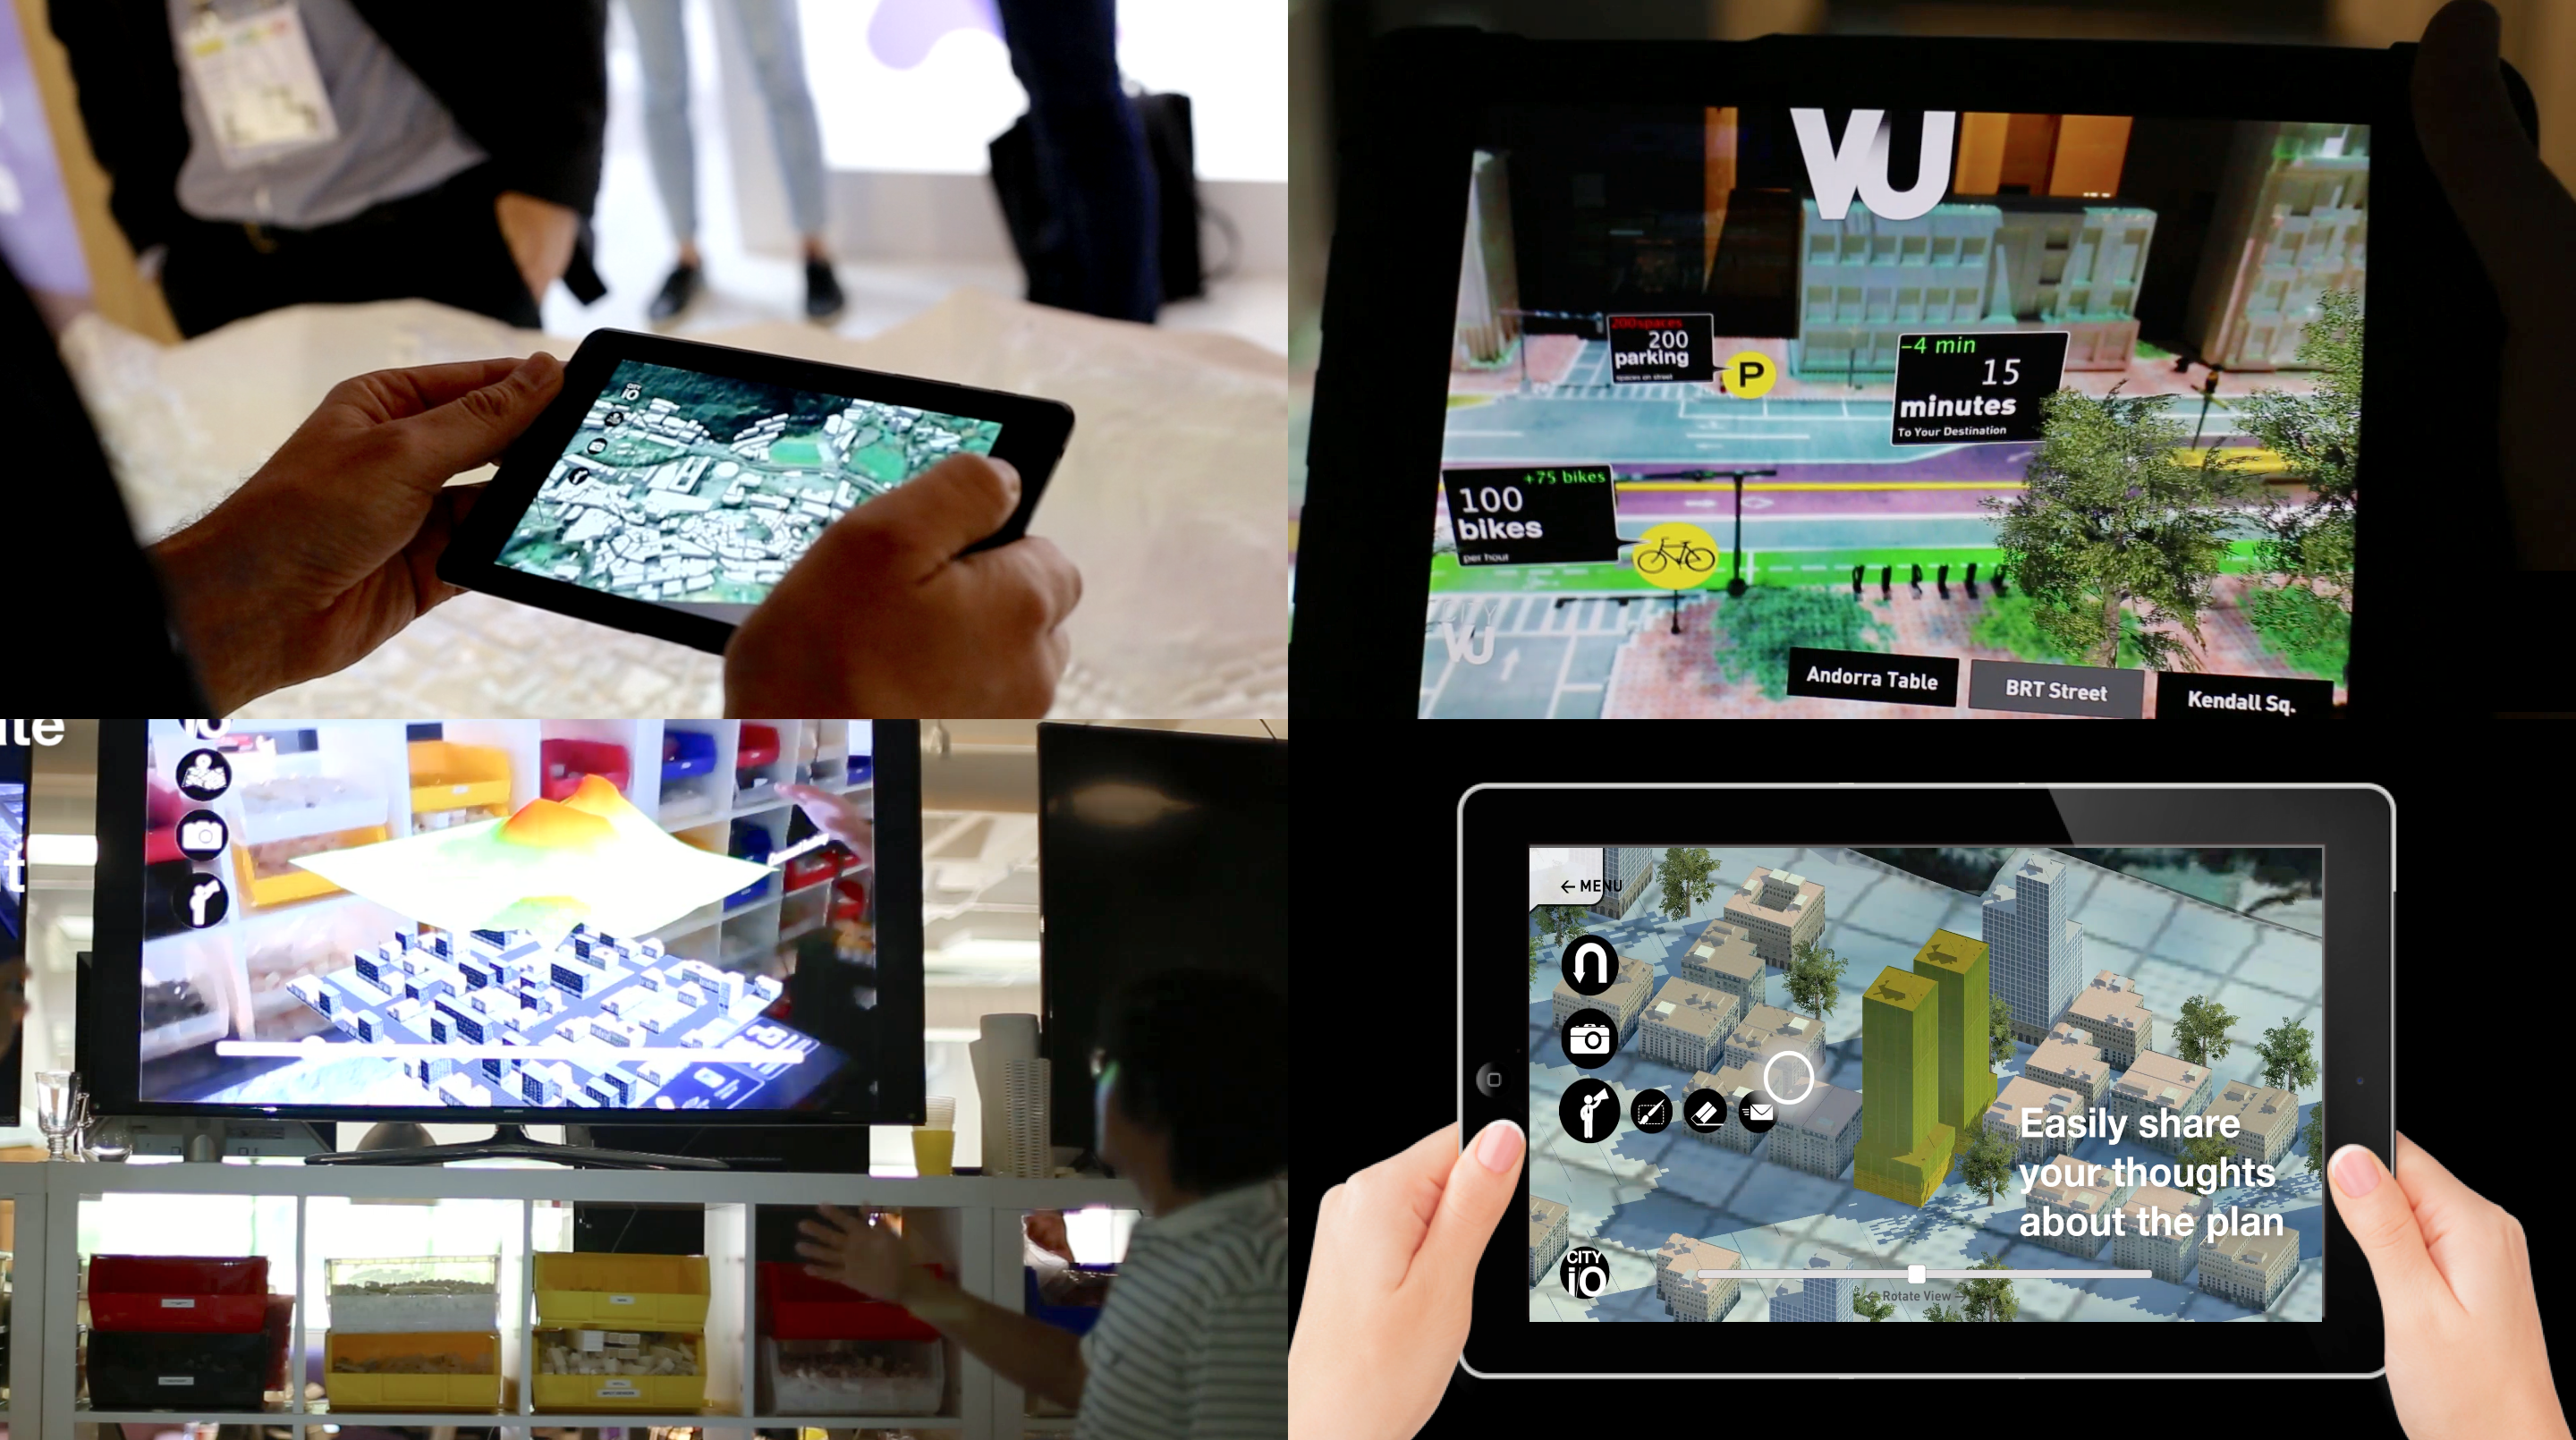
\includegraphics[width=1\textwidth]{chapters/transformation/cs_arch/figures/ar/ar_0.png}
              \end{center}
              \caption{CityScopeAR use-cases. (top-left) Andorra, in the Smart Cities conference, Barcelona \eqref{sec:andorra-data-observatory} ; (top-right) Boston BRT \eqref{sec:brt}; (bottom-left) Real-time interaction analysis with the TUI as a 3D heatmap; (bottom-right) Commenting interface for public engagement.}
              \label{fig:csar_world}
          \end{figure}


          \textbf{AndorrAR:} In 2016, a version of CityScopeAR was developed as part of a research collaboration in Andorra. Nicknamed `AnodrrAR', this variant was deployed at the Smart Cities conference in Barcelona, and later was set on permanent display at the Innovation Space in Caldea, Andorra la-Vella. AnodrrAR was designed as part of an interactive CityScope model which depicted several data layers: (i) Satellite imagery, 3D model of Andorra's landscape and urban areas designated for redevelopment; (ii) cell towers location, and simulation of the population interpreted from CDR data (see \eqref{sec:andorra-data-observatory}); (iii) interactive design proposals for the downtown area, collected from CityScope TUI via cityIO (see Section \eqref{subsec:csarch-cityio}). In this version, users could position and scale master-plans onto geo-located anchors in the virtual city model; and (iv) feedback system, allowing users to comment on urban developments using a virtual `Speech Bubble' interface.
          \newline
          During the Smart Cities conference in Barcelona, hundreds of visitors interacted with the tools, and over 200 feedback comments were recorded during each day of the event. Similar versions of CityScopeAR were deployed in Hamburg at the HCU university (`16), Volpe redevelopment site in Cambridge (`17) and in Shanghai, Tongji University (`17).
      }

      \subsubsection{CityScopeAR: Discussion}
      {
          CityScopeAR extends the CityScope process in terms of scale and location. It retains a linkage to the CityScope tangible interface, while augmenting it with on-demand data, analysis, and feedback. The feedback mechanism added a new layer to the CityScope ecosystem, allowing users to comment on urban development proposals, in a shared virtual or physical design session.
          \newline
          Despite its potential, AR technology is still relatively new, and has yet to reach mainstream usage \cite{mekni2014augmented}. CityScopeAR was an preliminary step towards adoption of AR technology for urban-design, but it also highlighted the challenges of the current state of the art. Specifically, cultivating a collaborative design process using individually hand-held devices was found to be a challenge. A major advantage of the CityScope TUI is in its ability to serve a common ground for conversation and feedback, unobstructed by devices. At the time of writing, even the most advanced AR or VR systems are still struggling with ease of use, accessability, comfort, and performance, hindering their mass use in a collaborative public setting.
      }
  }

  \subsection{Discussion}
  {

      This section discussed the various components of the CityScope ecosystem. It explored the CityScope Schema, a data structure and a standard used across the platform. It detailed the three main components of CityScope: (i) Input and interaction, (ii) urban analysis microservices, and (iii) feedback and visualizations. As a design decision, only few aspects of the CityScope ecosystem are immutable and fixed; Instead, the majority of the ecosystem is designed to be flexible and adaptable to the unique needs of the CityScope community, such as supporting a wide range of urban analytics modules, or the development of different input, visualization, and feedback modalities. The rest of this Chapter shows how this ecosystem was utilized in key CityScope projects.
  }
 }
